\documentclass[10pt]{book}
\usepackage[a6paper,hmargin=6.688mm,vmargin={17.736mm, 9.459mm}]{geometry}

% defn
\newenvironment{mdefn}{%
  \begin{figure}
    \begin{tcolorbox}
      \begin{defn}
        \raggedright
}{%
      \end{defn}
    \end{tcolorbox}
  \end{figure}
}
\newenvironment{idefn}{%
  \begin{figure}[htbp]
    \begin{tcolorbox}
      \begin{defn}
}{%
      \end{defn}
    \end{tcolorbox}
  \end{figure}
}

% floatbox
\newenvironment{mfloatbox}[1]{%
  \begin{figure}
    \begin{tcolorbox}
      \begin{floatbox}
        \begin{center}
          \bf #1
        \end{center}
}{%
      \end{floatbox}
    \end{tcolorbox}
  \end{figure}
}
\newenvironment{ifloatbox}[1]{%
  \begin{figure}
    \begin{tcolorbox}
      \begin{floatbox}
        \begin{center}
          \bf #1
        \end{center}
}{%
      \end{floatbox}
    \end{tcolorbox}
  \end{figure}
}

% thm
\newenvironment{mthm}{%
  \begin{figure}
    \begin{tcolorbox}
      \begin{thm}
}{%
      \end{thm}
    \end{tcolorbox}
  \end{figure}
}
\newenvironment{ithm}{%
  \begin{tcolorbox}
    \begin{thm}
}{%
    \end{thm}
  \end{tcolorbox}
}

% table
\newenvironment{mtable}{%
  \begin{table}
    \captionsetup{labelfont=bf,justification=centering}
    \begin{center}
}{%
    \end{center}
  \end{table}
}
\newenvironment{itable}{%
  \begin{table}[htp]
    \begin{center}
}{%
    \end{center}
  \end{table}
}

% figure
\newenvironment{mfigure}{%
  \begin{figure}
    \captionsetup{labelfont=bf,justification=centering}
    \begin{center}
}{%
    \end{center}
  \end{figure}
}
\newenvironment{ifigure}{%
  \begin{figure}[htp]
    \begin{center}
}{%
    \end{center}
  \end{figure}
}
% exinstr
\newcommand{\iexinstr}[1]{%
    \begin{tcolorbox}
      {#1}
    \end{tcolorbox}
}
\newcommand{\mexinstr}[1]{\iexinstr{#1}}

\newcommand{\sidenote}[1]{\footnote{#1}}

\usepackage{marginfix}
\usepackage[alerton,per=section,ragged]{sidenotesplus}
\usepackage{tabularx}
\usepackage{amssymb,amsmath,amsthm,fancyhdr,supertabular,longtable,hhline,mathtools}
\usepackage{colortbl}
\usepackage{import, multicol,boxedminipage}
\usepackage{chapterfolder}
\usepackage[metapost,truebbox]{mfpic}
\usepackage[pdflatex]{graphicx}
\usepackage{makeidx}
\usepackage{emptypage}

\usepackage{tikz-cd}

\usepackage{../shortlst}

\usepackage[colorlinks, hyperindex, plainpages=false, linkcolor=blue, urlcolor=blue, pdfpagelabels]{hyperref}
\let\oldhref\href
\renewcommand{\href}[2]{\oldhref{#1}{#2}\footnote{\url{#1}}}

\newcommand{\tabref}[1]{\hyperref[#1]{Table \ref{#1}}}

\usepackage[labelfont=bf]{caption}
\counterwithin{figure}{section}
\counterwithin{table}{section}
\usepackage[all]{hypcap}
\usepackage{bm}
\usepackage{braket}
\usepackage[normalem]{ulem}
\usepackage{enumitem}
\usepackage[skip=\medskipamount]{parskip}
\usepackage{pbox}
\usepackage[most]{tcolorbox}

\usepackage{tasks}
\usepackage{adjustbox}
\settasks{label=\arabic*., label-offset=0.6666em, label-width=14.1pt, counter=HW}

%% custom layout environments

% defn
\newenvironment{mdefn}{%
  \begin{marginfigure}
    \begin{tcolorbox}
      \begin{defn}
        \raggedright
}{%
      \end{defn}
    \end{tcolorbox}
  \end{marginfigure}
}
\newenvironment{idefn}{%
  \begin{figure}[htbp]
    \begin{tcolorbox}
      \begin{defn}
}{%
      \end{defn}
    \end{tcolorbox}
  \end{figure}
}
\newenvironment{fdefn}{%
  \begin{figure*}[tbp]
    \begin{tcolorbox}
      \begin{defn}
}{%
      \end{defn}
    \end{tcolorbox}
  \end{figure*}
}

% floatbox
\newenvironment{mfloatbox}[1]{%
  \begin{marginfigure}
    \begin{tcolorbox}
      \begin{floatbox}
        \begin{center}
          \bf #1
        \end{center}
}{%
      \end{floatbox}
    \end{tcolorbox}
  \end{marginfigure}
}
\newenvironment{ifloatbox}[1]{%
  \begin{figure}
    \begin{tcolorbox}
      \begin{floatbox}
        \begin{center}
          \bf #1
        \end{center}
}{%
      \end{floatbox}
    \end{tcolorbox}
  \end{figure}
}
\newenvironment{ffloatbox}[1]{%
  \begin{figure*}[tbp]
    \begin{tcolorbox}
      \begin{floatbox}
        \begin{center}
          \bf #1
        \end{center}
}{%
      \end{floatbox}
    \end{tcolorbox}
  \end{figure*}
}

% thm
\newenvironment{mthm}{%
  \begin{marginfigure}
    \begin{tcolorbox}
      \begin{thm}
}{%
      \end{thm}
    \end{tcolorbox}
  \end{marginfigure}
}
\newenvironment{ithm}{%
  \begin{tcolorbox}
    \begin{thm}
}{%
    \end{thm}
  \end{tcolorbox}
}
\newenvironment{fthm}{%
  \begin{figure}[!ht]
    \begin{tcolorbox}
      \begin{thm}
}{%
      \end{thm}
    \end{tcolorbox}
  \end{figure}
}

% table
\newenvironment{mtable}{%
  \begin{margintable}
    \captionsetup{labelfont=bf,justification=centering}
    \begin{center}
}{%
    \end{center}
  \end{margintable}
}
\newenvironment{ftable}{%
  \begin{table*}
    \begin{center}
}{%
    \end{center}
  \end{table*}
}
\newenvironment{itable}{%
  \begin{table}[htp]
    \begin{center}
}{%
    \end{center}
  \end{table}
}

% figure
\newbool{ismfigure}
\newenvironment{mfigure}{%
  \begin{marginfigure}
    \booltrue{ismfigure}
    \captionsetup{labelfont=bf,justification=centering}
    \begin{center}
}{%
    \end{center}
    \boolfalse{ismfigure}
  \end{marginfigure}
}
\newenvironment{ifigure}{%
  \begin{figure}[htp]
    \begin{center}
}{%
    \end{center}
  \end{figure}
}
\newenvironment{ffigure}{%
  \begin{figure}[tp]
    \begin{center}
}{%
    \end{center}
  \end{figure}
}

% graphtrans
\newenvironment{graphtrans}{%
  \begin{tikzcd}
}{%
  \end{tikzcd}
}
\newcommand{\trans}[1]{%
  \arrow[d, "\text{\parbox{20mm}{#1}}"] \\
}

\newcommand{\xincludegraphics}[1]{%
  \ifbool{ismfigure}{%
    \includegraphics[width=45mm]{#1}
  }{%
    \includegraphics[width=80mm]{#1}
  }
}
% xtcaption
\newcommand{\xtcaption}[1]{\tcaption{\parbox{40mm}{\centering\scriptsize #1}}}

% exinstr
\newcommand{\mexinstr}[1]{%
  \begin{marginfigure}
    \begin{tcolorbox}
      {\raggedright #1}
    \end{tcolorbox}
  \end{marginfigure}
}
\newcommand{\iexinstr}[1]{%
    \begin{tcolorbox}
      {#1}
    \end{tcolorbox}
}

\newcommand{\startexenum}{\setcounter{HW}{0}}

\newenvironment{exenum}{%
  \begin{enumerate}
  \setcounter{enumi}{\value{HW}}
}{%
  \setcounter{HW}{\value{enumi}}
  \end{enumerate}
}

\newenvironment{shortexenum}[1][\unskip]{%
  \begin{exenum}
}{%
  \end{exenum}
}


\newcommand{\transgraph}[2]{\stackrel{\text{\parbox{#1}{\centering \scriptsize #2}}}{\xrightarrow{\hspace{#1}}}}

\newcommand{\transgraphtwo}[3]{\stackrel{\transgraph{#1}{#2}}{\parbox{#1}{\centering \scriptsize #3}}}

\newenvironment{halfpage}{%
  \begin{minipage}{0.5\textwidth}
}{%
  \end{minipage}
}

\theoremstyle{definition}  % this prevents the text in definitions, theorems, and corollaries from being italicized
\newtheorem{floatbox}{\bf Box}[section]
\newcommand{\floatboxautorefname}{Box}
\newtheorem{defn}{\bf Definition}[section]
\newcommand{\defnautorefname}{Definition}
\newtheorem{thm}{\bf Theorem}[section]
\newcommand{\thmautorefname}{Theorem}
\newtheorem{cor}[thm]{\bf Corollary}
\newcommand{\corautorefname}{Corollary}
\newtheorem{eqn}{\bf Equation}[section]
\newcommand{\eqnautorefname}{Equation}

\newtheoremstyle{example-style}% 〈name〉
  {\medskipamount}%                      〈Space above〉
  {}%                       〈Space below〉
  {}%                  〈Body font〉
  {}%                          〈Indent amount〉
  {\bfseries}%                 〈Theorem head font〉
  {.}%                         〈Punctuation after theorem head〉
  { }%                         〈Space after theorem head〉
  {}%   
\theoremstyle{example-style}
\newtheorem{ex}{\bf Example}[section]
\newtheorem{fig}{\bf Figure}[section]

\setlength{\parindent}{0in}
\newcommand{\bbm}{\begin{boxedminipage}{\linewidth}}
\newcommand{\ebm}{\end{boxedminipage}}
\usepackage{array}
\setlength{\extrarowheight}{2pt}
\allowdisplaybreaks[2]
\usepackage{cancel}
\usepackage{sectsty}
%\usepackage{appendix}
\usepackage{textcomp}
\usepackage{multirow}
\usepackage[nottoc]{tocbibind}

\DeclareSymbolFont{AMSb}{U}{msb}{m}{n}
\DeclareMathSymbol{\C}{\mathbin}{AMSb}{"43}
\DeclareMathSymbol{\N}{\mathbin}{AMSb}{"4E}
\DeclareMathSymbol{\I}{\mathbin}{AMSb}{"5A}
\DeclareMathSymbol{\Q}{\mathbin}{AMSb}{"51}
\DeclareMathSymbol{\R}{\mathbin}{AMSb}{"52}
\DeclareMathSymbol{\W}{\mathbin}{AMSb}{"57}

\allsectionsfont{\mdseries \scshape}
\makeatletter
\renewcommand\l@section{\@dottedtocline{1}{1.5em}{3em}}
\renewcommand\l@subsection{\@dottedtocline{2}{4.5em}{3.5em}}
\makeatother
\pagestyle{fancy}
\newcounter{HW}
\newcounter{HWindent}

\renewcommand{\textinterrobang}{$! \! \! ?$}

%Below is for Iowna Font
%\renewcommand*\sfdefault{iwona}
%\usepackage[math]{iwona}

%Below is for Helvetica (scaled): 
\usepackage[scaled=.92]{helvet}   
\renewcommand{\familydefault}{\sfdefault}  %makes the text of the book sans serif
\usepackage[helvet]{sfmath}  %makes the math in the book sans serif
\allsectionsfont{\sffamily}  %makes the chapter and section titles sans serif

\makeatletter
\newcases{mycases}{\quad}{%
  \hfil$\m@th\displaystyle{##}$}{$\m@th\displaystyle{##}$\hfil}{\lbrace}{.}
\makeatother

\makeindex

\begin{document}

%removed \sc command from lines below.
\renewcommand{\chaptermark}[1]%
                  {\markboth{#1}{}}
\renewcommand{\sectionmark}[1]%
               {\markright{\thesection\ #1}}
\renewcommand{\headrulewidth}{0pt}
\lhead[\fancyplain{}{\thepage}]%
      {\fancyplain{}{\nouppercase{\rightmark}}}
\rhead[\fancyplain{}{\nouppercase{\leftmark}}]%
      {\fancyplain{}{\thepage}}
\cfoot{}
\fancypagestyle{plain}{\fancyhf{}}

\newgeometry{textwidth=130mm}
\frontmatter

\newcommand\sophia{
    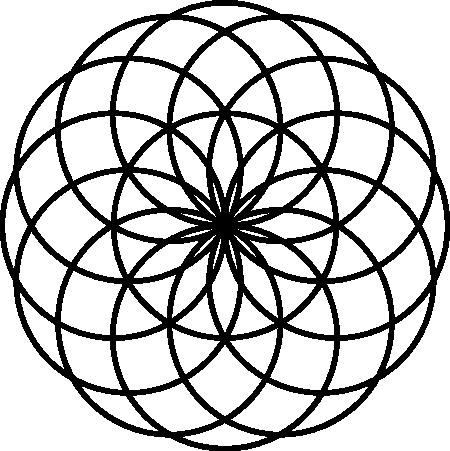
\includegraphics[width=18pt]{logo/logo.pdf}

    $\sigma o \phi \acute{\iota} \alpha$
}

\begin{titlepage}
\begin{center}

\vspace*{0.1\paperheight}

\Huge Precalculus --- Algebra II  \\ \vspace{.1in} \large Version $4 - \epsilon$  \\ \vspace{.25in} \large by

\vspace{0.1\paperheight}

\newcolumntype{Y}{>{\centering\arraybackslash}X}
\begin{tabularx}{0.953\linewidth}{YY} Carl Stitz, Ph.D. &  Jeff Zeager, Ph.D. \\ Lakeland Community College & Lorain County Community College \\\end{tabularx}

\vfill

\begin{center}
    \sophia
\end{center}

\end{center}
\end{titlepage}

% copyright page
\begingroup
\footnotesize
\setlength{\parindent}{0pt}
\setlength{\parskip}{\baselineskip}

\textcopyright{} 2025 Carl Stitz and Jeff Zeager \\
\url{https://stitz-zeager.com/}


\includegraphics[height=20pt]{../by-nc-sa.pdf}

This work is licensed under CC BY-NC-SA 3.0. To view a copy of this licence,
visit:

\url{https://creativecommons.org/licenses/by-nc-sa/3.0/deed.en}

\vfill

Sophia Publishing \\
\textsc{Chennai} \\
\url{https://sophia-publishing.github.io/} \\
\endgroup

%\include{acknowledgements}

\thispagestyle{empty}

\renewcommand{\contentsname}{Table of Contents}

\addtocontents{toc}{\protect\thispagestyle{empty}}

\clearpage

\pdfbookmark[1]{\contentsname}{toc}

\tableofcontents

%\chapter{Preface}
%\label{OldPreface}
%\thispagestyle{empty}
%Thank you for your interest in our book, but more importantly, thank you for taking the time to read the Preface.  I always read the Prefaces of the textbooks which I use in my classes because I believe it is in the Preface where I begin to understand the authors - who they are, what their motivation for writing the book was, and what they hope the reader will get out of reading the text.  Pedagogical issues such as content organization and how professors and students should best use a book can usually be gleaned out of its Table of Contents, but the reasons behind the choices authors make should be shared in the Preface.  Also, I feel that the Preface of a textbook should demonstrate the authors' love of their discipline and passion for teaching, so that I come away believing that they really want to help students and not just make money. Thus, I thank my fellow Preface-readers again for giving me the opportunity to share with you the need and vision which guided the creation of this book and passion which both Carl and I hold for Mathematics and the teaching of it.

Carl and I are natives of Northeast Ohio.  We met in graduate school at Kent State University in 1997.  I finished my Ph.D in Pure Mathematics in August 1998 and started teaching at Lorain County Community College in Elyria, Ohio just two days after graduation.  Carl earned his Ph.D in Pure Mathematics in August 2000 and started teaching at Lakeland Community College in Kirtland, Ohio that same month.  Our schools are fairly similar in size and mission and each serves a similar population of students.  The students range in age from about 16 (Ohio has a Post-Secondary Enrollment Option program which allows high school students to take college courses for free while still in high school.) to over 65.  Many of the ``non-traditional'' students are returning to school in order to change careers.  A majority of the students at both schools receive some sort of financial aid, be it scholarships from the schools' foundations, state-funded grants or federal financial aid like student loans, and many of them have lives busied by family and job demands.  Some will be taking their Associate degrees and entering (or re-entering) the workforce while others will be continuing on to a four-year college or university.  Despite their many differences, our students share one common attribute: they do not want to spend \$200 on a College Algebra book.

The challenge of reducing the cost of textbooks is one that many states, including Ohio, are taking quite seriously.  Indeed, state-level leaders have started to work with faculty from several of the colleges and universities in Ohio and with the major publishers as well.  That process will take considerable time so Carl and I came up with a plan of our own.  We decided that the best way to help our students right now was to write our own College Algebra book and give it away electronically for free.  We were granted sabbaticals from our respective institutions for the Spring semester of 2009 and actually began writing the textbook on December 16, 2008.  Using an open-source text editor called TexNicCenter and an open-source distribution of LaTeX called MikTex 2.7, Carl and I wrote and edited all of the text, exercises and answers and created all of the graphs (using Metapost within LaTeX) for Version $0.\overline{9}$ in about eight months.  (We choose to create a text in only black and white to keep printing costs to a minimum for those students who prefer a printed edition.  This somewhat Spartan page layout stands in sharp relief to the explosion of colors found in most other College Algebra texts, but neither Carl nor I believe the four-color print adds anything of value.)  I used the book in three sections of College Algebra at Lorain County Community College in the Fall of 2009 and Carl's colleague, Dr. Bill Previts, taught a section of College Algebra at Lakeland with the book that semester as well.  Students had the option of downloading the book as a .pdf file from our website \href{http://www.stitz-zeager.com}{www.stitz-zeager.com} or buying a low-cost printed version from our colleges' respective bookstores.  (By giving this book away for free electronically, we end the cycle of new editions appearing every 18 months to curtail the used book market.)  During Thanksgiving break in November 2009, many additional exercises written by Dr. Previts were added and the typographical errors found by our students and others were corrected. On December 10, 2009, Version $\sqrt{2}$ was released.  The book remains free for download at our website and by using \href{http://www.lulu.com/content/paperback-book/college-algebra/7513097}{Lulu.com} as an on-demand printing service, our bookstores are now able to provide a printed edition for just under \$19.  Neither Carl nor I have, or will ever, receive any royalties from the printed editions.    As a contribution back to the open-source community, all of the LaTeX files used to compile the book are available for free under a Creative Commons License on our website as well.  That way, anyone who would like to rearrange or edit the content for their classes can do so as long as it remains free.

The only disadvantage to not working for a publisher is that we don't have a paid editorial staff.  What we have instead, beyond ourselves, is friends, colleagues and unknown people in the open-source community who alert us to errors they find as they read the textbook.  What we gain in not having to report to a publisher so dramatically outweighs the lack of the paid staff that we have turned down every offer to publish our book.  (As of the writing of this Preface, we've had three offers.)  By maintaining this book by ourselves, Carl and I retain all creative control and keep the book our own.  We control the organization, depth and rigor of the content which means we can resist the pressure to diminish the rigor and homogenize the content so as to appeal to a mass market.  A casual glance through the Table of Contents of most of the major publishers' College Algebra books reveals nearly isomorphic content in both order and depth.   Our Table of Contents shows a different approach, one that might be labeled ``Functions First.''  To truly use The Rule of Four, that is, in order to discuss each new concept algebraically, graphically, numerically and verbally, it seems completely obvious to us that one would need to introduce functions first.  (Take a moment and compare our ordering to the classic ``equations first, then the Cartesian Plane and THEN functions'' approach seen in most of the major players.)  We then introduce a class of functions and discuss the equations, inequalities (with a heavy emphasis on sign diagrams) and applications which involve functions in that class.  The material is presented at a level that definitely prepares a student for Calculus while giving them relevant Mathematics which can be used in other classes as well.  Graphing calculators are used sparingly and only as a tool to enhance the Mathematics, not to replace it.  The answers to nearly all of the computational homework exercises are given in the text and we have gone to great lengths to write some very thought provoking discussion questions whose answers are not given.  One will notice that our exercise sets are much shorter than the traditional sets of nearly 100 ``drill and kill'' questions which build skill devoid of understanding.  Our experience has been that students can do about 15-20 homework exercises a night so we very carefully chose smaller sets of questions which cover all of the necessary skills and get the students thinking more deeply about the Mathematics involved.

Critics of the Open Educational Resource movement might quip that ``open-source is where bad content goes to die,'' to which I say this: take a serious look at what we offer our students.  Look through a few sections to see if what we've written is bad content in your opinion.  I see this open-source book not as something which is ``free and worth every penny'', but rather, as a high quality alternative to the business as usual of the textbook industry and I hope that you agree.  If you have any comments, questions or concerns please feel free to contact me at jeff@stitz-zeager.com or Carl at carl@stitz-zeager.com.

\bigskip

\hfill \pbox{\textwidth}{Jeff Zeager\\Lorain County Community College\\January 25, 2010}

%\chapter{The New Preface}
%\label{NewPreface}
%\thispagestyle{empty}
%\input{NewPreface}

\mainmatter
 

\renewcommand{\chaptername}{Chapter}

\restoregeometry

%\chapter{Introduction to Functions}
%\label{IntroductiontoFunctions}
%\thispagestyle{empty}
%\import{../IntroductiontoFunctions/}{IntroductiontoFunctions}

%\chapter{Polynomial Functions}
%\label{PolynomialFunctions}
%\thispagestyle{empty}
%\import{../PolynomialFunctions/}{PolynomialFunctions}

\chapter{Rational Functions}
\label{RationalFunctions}
\thispagestyle{empty}
\import{../RationalFunctions/}{RationalFunctions}

\chapter{Root, Radical and Power Functions}
\label{RootRadicalPowerFunctions}
\thispagestyle{empty}
\import{../RootRadicalPowerFunctions/}{RootRadicalPowerFunctions}

\chapter{Further Topics on Functions}
\label{FurtherTopicsonFunctions}
\thispagestyle{empty}
\import{../FurtherTopicsonFunctions/}{FurtherTopicsonFunctions}

%\chapter{Exponential and Logarithmic Functions}
%\label{ExponentialandLogarithmicFunctions}
%\thispagestyle{empty}
%\import{../ExponentialandLogarithmicFunctions/}{ExponentialandLogarithmicFunctions}

% \chapter{The Conic Sections}
% \label{TheConicSections}
% \thispagestyle{empty}
% \import{./TheConicSections/}{TheConicSections}

% \chapter{Systems of Equations and Matrices}
% \label{SystemsofEquationsandMatrices}
% \thispagestyle{empty}
% \import{./SystemsofEquationsandMatrices/}{SystemsofEquationsandMatrices}

% \chapter{Sequences and the Binomial Theorem}
% \label{SequencesandtheBinomialTheorem}
% \thispagestyle{empty}
% \import{./SequencesandtheBinomialTheorem/}{SequencesandtheBinomialTheorem}

% \chapter{Foundations of Trigonometry}
% \label{FoundationsofTrigonometry}
% \thispagestyle{empty}
% \import{./FoundationsofTrigonometry/}{FoundationsofTrigonometry}

% \chapter{Analytical Trigonometry}
% \label{AnalyticalTrigonometry}
% \thispagestyle{empty}
% \import{./AnalyticalTrigonometry/}{AnalyticalTrigonometry}

% \chapter{Geometric Applications of Trigonometry}
% \label{GeometricApplicationsofTrigonometry}
% \thispagestyle{empty}
% \import{./GeometricApplicationsofTrigonometry/}{GeometricApplicationsofTrigonometry}

% \chapter{Polar Coordinates and Parametric Equations}
% \label{PolarCoordinatesandParametricEquations}
% \thispagestyle{empty}
% \import{./PolarCoordinatesandParametricEquations/}{PolarCoordinatesandParametricEquations}

\backmatter

\let\originalstyle=\thispagestyle            % Store the command for later reuse.
%\def\thispagestyle#1{\fancyfoot[C]{}}       % This clears footer in the center if fancyhdr is in use.
\def\thispagestyle#1{\originalstyle{empty}} % Use this to get blank header+footer, TeXnically it is only \thispagestyle{empty}.
%\def\thispagestyle#1{}                       % This line completely ignores the content of the \thispagestyle command.
\printindex                                  % Typeset the actual Index.
\let\thispagestyle=\originalstyle            % Let's get back to the original version of the \thispagestyle, if needed later in the document.



\end{document}
